%%%%%%%%%%%%%%%%%%%%%%%%%%%%%%%%%%%%%%%%%
% Wenneker Article
% LaTeX Template
% Version 2.0 (28/2/17)
%
% This template was downloaded from:
% http://www.LaTeXTemplates.com
%
% Authors:
% Vel (vel@LaTeXTemplates.com)
% Frits Wenneker
%
% License:
% CC BY-NC-SA 3.0 (http://creativecommons.org/licenses/by-nc-sa/3.0/)
%
%%%%%%%%%%%%%%%%%%%%%%%%%%%%%%%%%%%%%%%%%

%----------------------------------------------------------------------------------------
%	PACKAGES AND OTHER DOCUMENT CONFIGURATIONS
%----------------------------------------------------------------------------------------

\documentclass[10pt, a4paper, twocolumn]{article} % 10pt font size (11 and 12 also possible), A4 paper (letterpaper for US letter) and two column layout (remove for one column)

%%%%%%%%%%%%%%%%%%%%%%%%%%%%%%%%%%%%%%%%%
% Wenneker Article
% Structure Specification File
% Version 1.0 (28/2/17)
%
% This file originates from:
% http://www.LaTeXTemplates.com
%
% Authors:
% Frits Wenneker
% Vel (vel@LaTeXTemplates.com)
%
% License:
% CC BY-NC-SA 3.0 (http://creativecommons.org/licenses/by-nc-sa/3.0/)
%
%%%%%%%%%%%%%%%%%%%%%%%%%%%%%%%%%%%%%%%%%

%----------------------------------------------------------------------------------------
%	PACKAGES AND OTHER DOCUMENT CONFIGURATIONS
%----------------------------------------------------------------------------------------

\usepackage[english]{babel} % English language hyphenation

\usepackage{microtype} % Better typography

\usepackage{amsmath,amsfonts,amsthm} % Math packages for equations

\usepackage[svgnames]{xcolor} % Enabling colors by their 'svgnames'

\usepackage[hang, small, labelfont=bf, up, textfont=it]{caption} % Custom captions under/above tables and figures

\usepackage{booktabs} % Horizontal rules in tables

\usepackage{lastpage} % Used to determine the number of pages in the document (for "Page X of Total")

\usepackage{graphicx} % Required for adding images

\usepackage{enumitem} % Required for customising lists
\setlist{noitemsep} % Remove spacing between bullet/numbered list elements

\usepackage{sectsty} % Enables custom section titles
\allsectionsfont{\usefont{OT1}{phv}{b}{n}} % Change the font of all section commands (Helvetica)

\usepackage{hyperref}
\usepackage{url}
\usepackage{cleveref}
\usepackage{float}
\newtheorem{theorem}{Theorem}[section]
\newtheorem{lemma}[theorem]{Lemma}
\crefname{lemma}{lemma}{lemmas}
\numberwithin{equation}{section}
\counterwithin{figure}{section}

%----------------------------------------------------------------------------------------
%	MARGINS AND SPACING
%----------------------------------------------------------------------------------------

\usepackage{geometry} % Required for adjusting page dimensions

\geometry{
	top=1cm, % Top margin
	bottom=1.5cm, % Bottom margin
	left=2cm, % Left margin
	right=2cm, % Right margin
	includehead, % Include space for a header
	includefoot, % Include space for a footer
	%showframe, % Uncomment to show how the type block is set on the page
}

\setlength{\columnsep}{7mm} % Column separation width

%----------------------------------------------------------------------------------------
%	FONTS
%----------------------------------------------------------------------------------------

\usepackage[T1]{fontenc} % Output font encoding for international characters
\usepackage[utf8]{inputenc} % Required for inputting international characters

\usepackage{XCharter} % Use the XCharter font

%----------------------------------------------------------------------------------------
%	HEADERS AND FOOTERS
%----------------------------------------------------------------------------------------

\usepackage{fancyhdr} % Needed to define custom headers/footers
\pagestyle{fancy} % Enables the custom headers/footers

\renewcommand{\headrulewidth}{0.0pt} % No header rule
\renewcommand{\footrulewidth}{0.4pt} % Thin footer rule

\renewcommand{\sectionmark}[1]{\markboth{#1}{}} % Removes the section number from the header when \leftmark is used

%\nouppercase\leftmark % Add this to one of the lines below if you want a section title in the header/footer

% Headers
\lhead{} % Left header
%\chead{\textit{\thetitle}} % Center header - currently printing the article title
\rhead{} % Right header

% Footers
\lfoot{} % Left footer
\cfoot{} % Center footer
\rfoot{\footnotesize Page \thepage\ of \pageref{LastPage}} % Right footer, "Page 1 of 2"

\fancypagestyle{firstpage}{ % Page style for the first page with the title
	\fancyhf{}
        \rfoot{\footnotesize Page \thepage\ of \pageref{LastPage}}
}

%----------------------------------------------------------------------------------------
%	TITLE SECTION
%----------------------------------------------------------------------------------------

\newcommand{\authorstyle}[1]{{\large\usefont{OT1}{phv}{b}{n}\color{Black}#1}} % Authors style (Helvetica)

\newcommand{\universitymail}[1]{{\small\usefont{OT1}{phv}{b}{n}\color{Black}#1}} % Authors style (Helvetica)

\usepackage{titling} % Allows custom title configuration

\newcommand{\HorRule}{\color{DarkGoldenrod}\rule{\linewidth}{1pt}} % Defines the gold horizontal rule around the title
\iffalse
\pretitle{
	\vspace{-50pt} % Move the entire title section up
	\fontsize{32}{36}\usefont{OT1}{phv}{b}{n}\selectfont % Helvetica
	\color{Black} % Text colour for the title and author(s)
}

\posttitle{\par\vskip 10pt} % Whitespace under the title

\preauthor{} % Anything that will appear before \author is printed

\postauthor{ % Anything that will appear after \author is printed
	\vspace{10pt} % Space before the rule
	\vspace{10pt} % Space after the title section
        \begin{center}
\includegraphics[width=0.16\textwidth]{unipi.png}\end{center}
}
\fi

%----------------------------------------------------------------------------------------
%	BIBLIOGRAPHY
%----------------------------------------------------------------------------------------
\usepackage{natbib}
%\usepackage[backend=bibtex,style=authoryear,natbib=true]{biblatex} % Use the bibtex backend with the authoryear citation style (which resembles APA)

%\addbibresource{references.bib} % The filename of the bibliography

\usepackage[autostyle=true]{csquotes} % Required to generate language-dependent quotes in the bibliography
 % Specifies the document structure and loads requires packages

%----------------------------------------------------------------------------------------
%	ARTICLE INFORMATION
%----------------------------------------------------------------------------------------
\title{\vspace{-2cm}\textbf{PokéBOT, a Pokémon battle bot}}
\author{\textbf{\small{\textit{Dalla Noce Niko, Lombardi Giuseppe, Ristori Alessandro}}} \\ % put your full name here
        \small{Master Degree in Computer science.}\\ \small{\{n.dallanoce, g.lombardi11, a.ristori5\}@studenti.unipi.it} \\  % put your Master Degree here
        \small{Artificial intelligence fundamentals, Academic Year: 2022/2023} \\
        \textbf{\small{\url{https://github.com/nikodallanoce/PokeBOT}}} \\ \\
        
\includegraphics[width=0.10\textwidth]{unipi.png}
}

% Example of a one line author/institution relationship
\date{\small{\today}} % Add a date here if you would like one to appear underneath the title block, use \today for the current date, leave empty for no date

%----------------------------------------------------------------------------------------

\begin{document}
\newcommand{\poke}{\textit{Pokémon}\space}

\maketitle % Print the title


\thispagestyle{firstpage} % Apply the page style for the first page (no headers and footers)
\raggedbottom

%----------------------------------------------------------------------------------------
%	ARTICLE CONTENTS
%----------------------------------------------------------------------------------------

\section{Introduction}\label{sec:introduction}
In the AI field, games have always been given a soft spot since they are ideal as first tests for AI algorithms and they provide a variety of environments
in which rules are well-defined and can be exploited in order to understand the complexity of such environments and how to apply the same reasoning on harder research fields. For such reason, and for giving nostalgia another ride, we decided to focus our work on \poke battles.

\poke battles are an interesting \textit{multi-agent non-cooperative} environment in which two players have six \poke each and their goal is to defeat all the opponent's \textit{Pokémon}. Battles are based on atomic turns that are defined as the two moves chosen by the players and resolved simultaneously, such moves can fail given a probability called \textit{accuracy} and their \textit{secondary effects} have an impact on the next turns, for this reason the environment under consideration is also \textit{partially deterministic} and \textit{not episodic}.
Moreover, both players do not have perfect knowledge of the environment and they can use this fact in order to gain an advantage over the opponent by switching out the active \poke or revealing a move or item that was not shown before.

Our aim is not to build the perfect \poke battle bot (which is near to impossible given the stochasticity of this environment), but to build one that can stand its own against human players.

\section{Related works}\label{sec:relatedworks}
All of our players were thought to be developed in order to run on an online open-source \poke battle simulator \cite{remote_server} which was also vital for the performance's evaluation of our bot.

For that reason, our work was mainly inspired by \cite{showdown_competition}, starting from that we looked for more implementations in order to give ourselves an overall idea about what to do. During our research we found the poke-env library \cite{poke_env} which gave us a very useful engine and some \textit{baseline} players that were essential for testing ours; the strongest baseline player of the library was the main metric of comparison of our work.

The choice of players was, instead, based on implementations found on \textit{Github}, where we have found a small, but working, example of rule-based and minimax players \cite{rempton} and a bot that is considered among the best ones in the online community \cite{pmariglia}. The former is built on the poke-env library \cite{poke_env}, so we used it for defining the structure of our players, while the latter gave us ideas on how to improve the stats and damage computations.

\section{Methodologies}\label{sec:methodologies}
Just like \poke evolve upon reaching certain conditions, we applied the same reasoning for the development of our bot. First of all we started with a simple player (called \textit{MaxBasePower} or \textit{MBP}) that chooses the non-status move with the highest base power, regardless of the actual damage dealt. Then, we upgraded this first simple player by letting it choose the move with the highest actual damage thanks to a hand-crafted stats and damage computations (we called this player as \textit{BestDamage} or \textit{BD}).

The damage computation is the main engine of our bot, since the more accurate is the damage dealt the higher the performance of the players.

\begin{multline} 
    damage = \left (\frac{(\frac{2\times level}{5} + 2) \times power \times A/D}{50} + 2 \right) \\ \times targets \times PB \times weather \times critical \\ \times random \times STAB \times type \times burn \times other
\label{eq:damage}   
\end{multline}

As we can see from \eqref{eq:damage}, the damage computation is made up of many parameters and each one of them contains several rules that can be explained in FOL, an example is shown in \eqref{eq:rule}.
\begin{multline}
    \forall x \hspace{1mm} \poke(x) \wedge \forall y \hspace{1mm} Move(y) \wedge Holds(x,airbaloon) \\
    \wedge MoveType(y,Ground) \Rightarrow Immune(x,y)
    \label{eq:rule}
\end{multline}

After finishing the engine, we had to deal with switches; the main issue with them is that there is not an optimal number and the situations in which we should use this mechanic can not be hard-coded since they would be too many. To alleviate all of this, we decided to build what we have called a \textit{matchup} function that, given the two \poke, computes the advantage (or disadvantage) the bot has. The computation of the \textit{matchup} value for each not fainted bot's \poke is based on the damage multipliers coming from their types and moves:
\begin{enumerate}
    \item First we take the max damage multiplier based on types for both the bot's and opponent's \poke as shown in \autoref{fig:damage_multipliers}.
    \item Then, we compute the difference between the two values obtaining what we called the \textit{type advantage}.
    \item We do the same for the moves, in case the opponent's \poke has no known moves we suppose that it will have at least one move for each one of its types and we assign it a default move.
    \item Just like we did for the types we do the same difference to compute the \textit{move advantage}
    \item At the end, we sum both values to obtain the actual \textit{matchup} $\in [-8,8]$ which indicates how favourable is the current situation for the bot's \poke against the opponent's.
\end{enumerate}
\begin{figure}[!htbp]
    \centering
    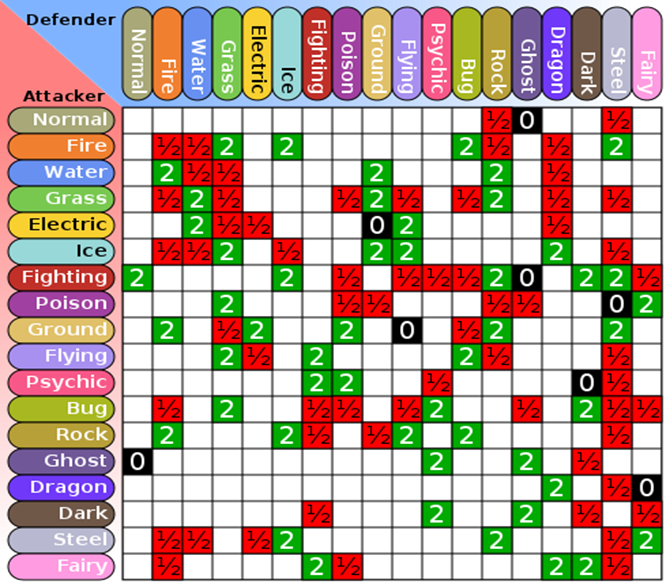
\includegraphics[width=0.8\linewidth]{images/damage_multipliers.png}
    \caption{Damage multipliers for each type}
    \label{fig:damage_multipliers}
\end{figure}

\subsection{Rule-Based Player}\label{subsec:rule_based_player}
The first enhanced version of our bot is the rule-based player (or \textit{RB}) which uses everything we talked about until now plus some more improvements thanks to an external expert. We defined even more rules to deal with \textit{healing}, \textit{status}, \textit{boost}, \textit{protective} and \textit{retaliatory} moves, while also implementing a strategy for deciding when to switch out and under which situations we should use the gimmick, which is dynamax for the generation our bot will play in.

\subsection{MiniMax Player}\label{subsec:minimax_player}
The second enhanced player we developed uses the minimax algorithm with $\alpha$-$\beta$ pruning in order to choose the best action to take (we called such player as \textit{MiniMax} or \textit{MM}). Generally, a player can choose either to make a move or to switch out the active \textit{Pokémon}, for this reason, the mini-max tree has a branching factor that is the sum of the number of available moves of the active \poke and the number of available switches; the latter are, usually, the number of not fainted \poke in a team.

The root node of a tree represents the actual current state of a battle that we want to start simulating, in which we assume the bot to take an action first i.e. before the opponent player. The depth of the tree is two time the turns we want to simulate because in a \poke battle, a turn ends when both the players have chosen an action. In this way, assuming $t$ is the turn we want to simulate, the effects of our actions are computed at each $2t + 1$ depth level, while the opponent ones at every $2t$, with $t>0$, depth level. Taking into account everything we have seen until now we can say that each one of the nodes simulates the progress of a battle, as an example, see \autoref{fig:minimax_with_switches}.

As we first said in \autoref{sec:introduction}, a \poke battle is a partially observable environment in which the opponent’s team, \poke statistics, abilities and moves can not be known a priori and each move has its own probability to hit. As a consequence, the library \cite{poke_env} does not allow to simulate the progress of a battle, otherwise it would have been like cheating. To overcome these limitations, at the beginning of each battle, we build a knowledge base that is composed by the \poke that belong to our team and all their attributes plus the opponent's active \textit{Pokémon}. Whenever the opponent player chooses a move or switches to a \textit{Pokémon}, we add these information to the knowledge base in order to simulate the progress of the battle more accurately as possible. It is not possible to consider all the variables of a battle, so the most relevant ones we considered are: the weather conditions, the moves, statistics and boosts of both active \poke and finally, the composition of our team and the opponent's. All these variables may change from turn to turn assuming a crucial role when computing the damage, the recoil or the drain of a move. Then, in order to know whether or not we are at an advantage over the opponent, we developed an heuristic.

\subsection{Heuristic}\label{subsec:heuristic}
To estimate the utility of a node, we use an heuristic that uses knowledge of the current state to tell us how favourable is a particular battle progress.

Initially, we used a straightforward evaluation function that uses only the knowledge of both active \poke: we considered the ratio of the current hp (health points) of the \poke over its max hp \eqref{eq:simple_heuristic}.
\begin{multline}
    f(node)=\bar{hp}\left(active_{Bot}\right)-\bar{hp}\left(active_{Opp}\right)
    \label{eq:simple_heuristic}
\end{multline}
The minimax algorithm with such function has some limitations since it has no global knowledge about the state of the game: as an example, the opponent's active \poke might be defeated, but all the remaining \poke of his team are alive; in this case, the rating function gives a very positive score even if our team has only one not fainted \poke.

Considering these limits, we decided to use a more reliable function that considers the ratio between the hp of the entire team and the number of surviving \poke. Finally, we added a penalty term on the depth of the node to the evaluation function \cite{showdown_competition}; this penalty promotes exploration among all possible strategies and discourages excessive turn depth.
The resulting evaluation function is a linear weighted sum \eqref{eq:complex_heuristic} where the weight of each term indicates how relevant the term is to the state evaluation. By defying $alive(team)= num \; of \; \text{\textit{Pokémon}} \; alive \; in \; the \; team$, the evaluation function can be written as:

\begin{equation}
\begin{split}
    f(node)&=w_1 \cdot \bar{hp}(team_{Bot}) +w_2 \cdot alive\left(team_{Bot}\right) \\ 
    & - w_3 \cdot \bar{hp}\left(team_{Opp}\right)
    - w_4 \cdot alive\left(team_{Opp}\right) \\
    &-w_5 \cdot depth(node)
\end{split}
\label{eq:complex_heuristic}
\end{equation}
We performed a random search on the weights to find the best configuration of the function and evaluated each configuration by observing the minimax player's performances. The best-resulting weights configuration favours dealing damage to the opposing Pokemon rather than rewarding survival and associates a small depth penalty.

\section{Assessment}\label{sec:assessment}
In order to evaluate the strength of our different player strategies, we first ran them in a local server, a feature implemented in \cite{poke_env}, that simulates a player vs player battle. It did not work out of the box due to some incompatibilities between the Node JS version and the Python one, so, in order to solve this problem and to improve reproducibility, we wrote a Docker \cite{merkel2014docker} file that is available in the root of the GitHub repository. The poke-env library \cite{poke_env} implements a "baseline" player that has an Elo rank of 1100-1200 points on the remote server \cite{showdown_competition}. So, our aim was to develop at least two players, a rule-based (\autoref{subsec:rule_based_player}) and a minimax (\autoref{subsec:minimax_player}), that could defeat it. Then, we made them battle against each other a thousand of times to assess their strength. At this point, it faced out that the mini-max player made too many \poke switches, so we developed a new strategy in which we exclude them from the mini-max tree computation. In \autoref{fig:minimax_without_switches} we can see the differences with respect to the approach described in \autoref{subsec:minimax_player}. In this way, the player chooses whether or not switch a \poke at the beginning of each turn, only based on the matchup score, just like the rule-based player does.

So, going back to performances between each player, we can declare, by looking at \autoref{tab:win_percentage_players}, the rule-based and minimax players to be the best ones as expected.
\begin{table}[!htbp]
    \footnotesize
    \centering
    \begin{tabular}{c|c|c|c|c}
        \hline \hline
         \textbf{Player} & \textbf{MBP} & \textbf{BD} & \textbf{RB} & \textbf{MM} \\ \hline \hline
         \textbf{MBP} & / & 0.104 & 0.084 & 0.114 \\ \hline
         \textbf{BD} & 0.896 & / & 0.398 & 0.452 \\ \hline
         \textbf{RB} & 0.916 & 0.602 & / & 0.571 \\ \hline
         \textbf{MM} & 0.886 & 0.548 & 0.429 & / \\ \hline \hline
    \end{tabular}
    \caption{Percentage of win for every player against each other}
    \label{tab:win_percentage_players}
\end{table}

We have also noticed some more things: first of all using the matchup function for choosing the best switch increased the performance of about $5\%$ (with a proper switch strategy of course) against the baseline player from \cite{poke_env}, while using the gimmick strategy had the major effect with a $8$-$9\%$ increase in performance.

As a final test, we run our two best players for $100$ matches on the remote server \cite{remote_server} against human players on generation $8$ random battles. We can look at their ELO progression in \autoref{fig:elo_players}.
\begin{figure}[!htbp]
    \centering
    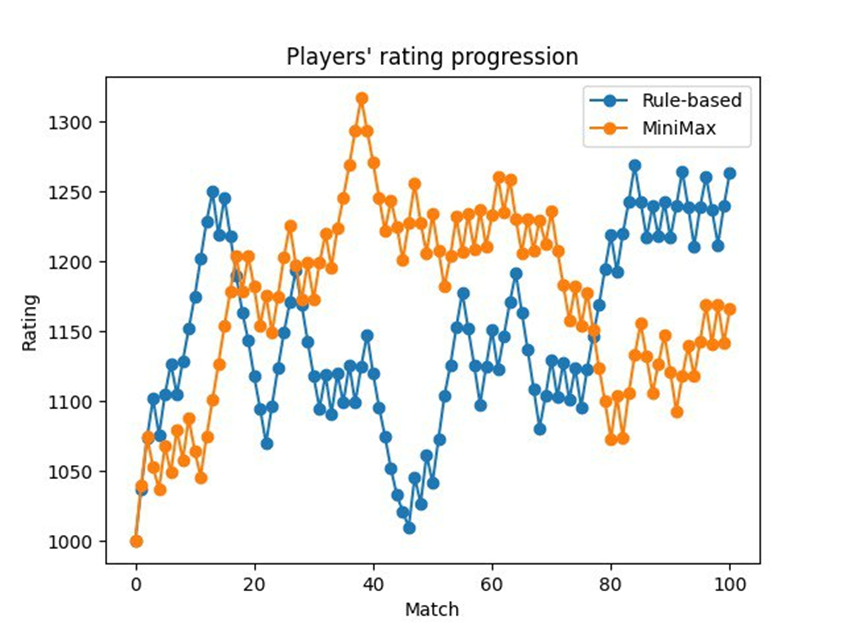
\includegraphics[width=0.8\linewidth]{images/elo_players.png}
    \caption{ELO progression of RB and MM players against human players}
    \label{fig:elo_players}
\end{figure}
It turns out that the two players float around the $1200$ ELO points, making them somewhat at the level of an average skilled human player.

\section{Conclusion}\label{sec:conclusion}
Building a \poke battle bot proved to be an exciting and motivating challenge and this project allowed us to apply some artificial intelligence methods, especially those regarding game theory and adversarial agents. 
We overcame many difficulties while "evolving" our bot and its gradual refinement, that ended up in two different but near equally strong players, has resulted in an artificial "trainer" with the strength and behaviour of an average skilled human player, which was our initial aim.

%-------------------------------------------------------------------------------
%	BIBLIOGRAPHY
%-------------------------------------------------------------------------------
\newpage
\onecolumn
\setcitestyle{square}
\bibliographystyle{plain}
\bibliography{references}

%-------------------------------------------------------------------------------
\newpage
\appendix
\section{Appendix}\label{sec:appendix}
\subsection{Team contributions}\label{appendix:team_contributions}
\begin{itemize}
    \item \textbf{Niko:} setup of local server, minimax player, $\alpha$-$\beta$ pruning and heuristics.
    \item \textbf{Giuseppe:} gimmick rules, $\alpha$-$\beta$ pruning, heuristics and scripts for running the players.
    \item \textbf{Alessandro:} stats and damage computation, baseline players, matchup rules and rule-based player.
\end{itemize}

\subsection{Github metrics}\label{appendix:github_metrics}
\begin{table}[!htbp]
    \footnotesize
    \centering
    \begin{tabular}{c|c|c}
        \hline \hline
         \textbf{Member} & \textbf{Commits} & \textbf{Major activity period} \\ \hline \hline
         Niko & 63 & middle of november \\ \hline
         Giuseppe & 45 & middle of november \\ \hline
         Alessandro & 71 & start of november \\ \hline \hline
    \end{tabular}
    \caption{Github contributions for each member}
    \label{tab:git_contributions}
\end{table}

\subsection{Relationship with the course}\label{appendix:course_relationship}
\begin{itemize}
    \item Study and definition of the problem:
    \begin{itemize}
        \item Definition of the environment and its characteristics.
        \item Definition of the type of game.
        \item Acting under uncertainty.
    \end{itemize}
    \item Definition of the agents:
    \begin{itemize}
        \item Logical agent (Rule-based)
            \begin{itemize}
            \item Definition of rules in FOL.
            \end{itemize}
        \item MiniMax algorithm
            \begin{itemize}
            \item $\alpha$-$\beta$ pruning.
            \item Definition of the Heuristic function.
            \end{itemize}
    \end{itemize}
    \item Exploit non-cooperative Game Theory:
    \begin{itemize}
        \item Weak dominant strategy for type matchup.
    \end{itemize}
    
\end{itemize}

\subsection{Mini-max tree}
\begin{figure}[H]
    \centering
    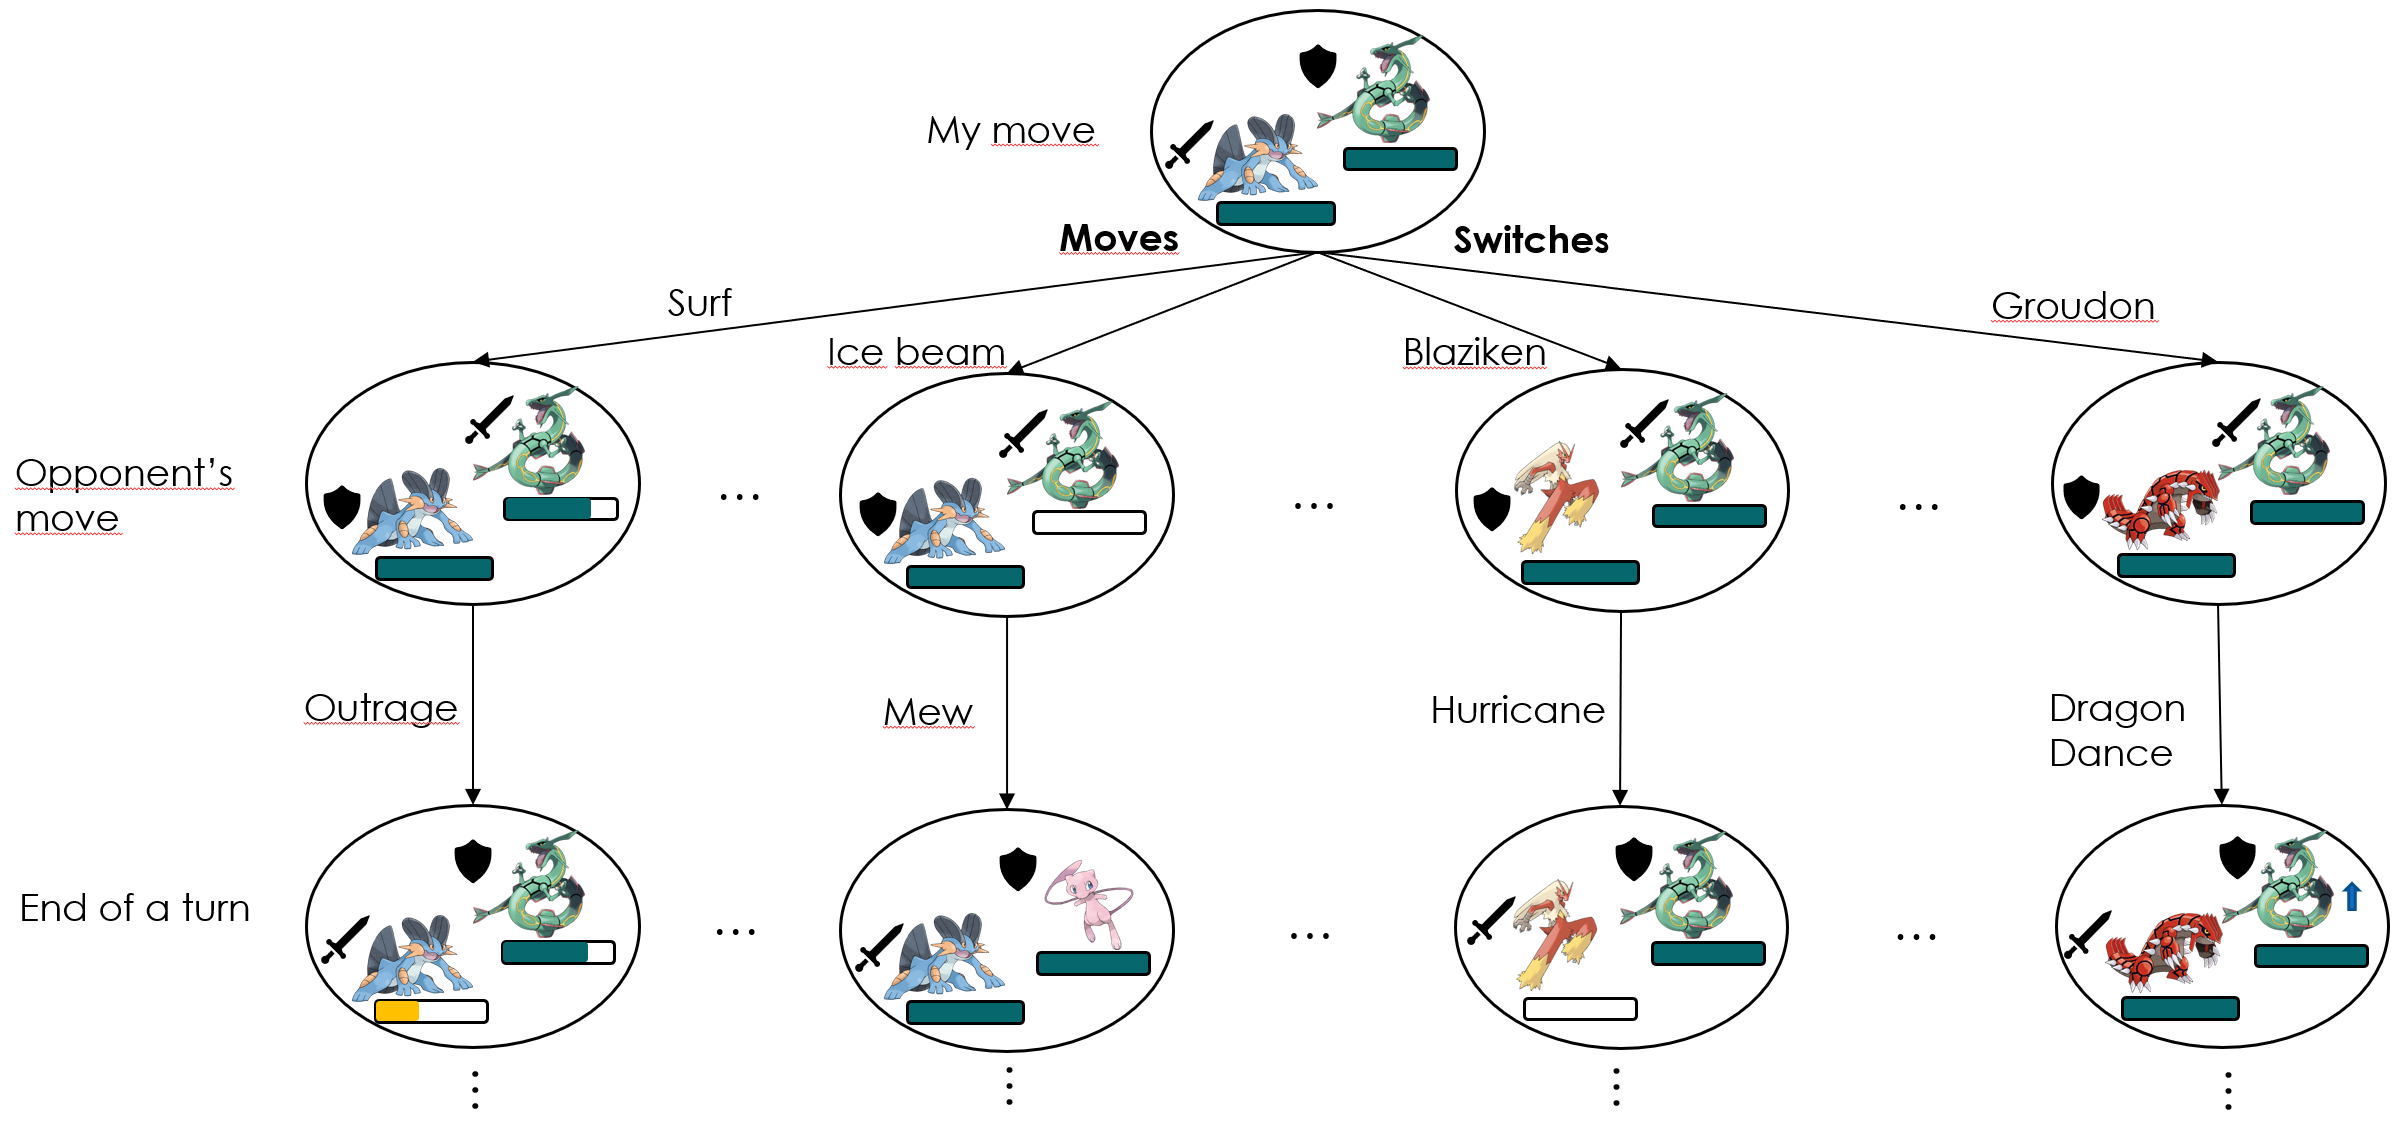
\includegraphics[width=0.8\textwidth]{images/minimax with switches.png}
    \caption{Minimax tree with switches.}
    \label{fig:minimax_with_switches}
\end{figure}

\begin{figure}[H]
    \centering
    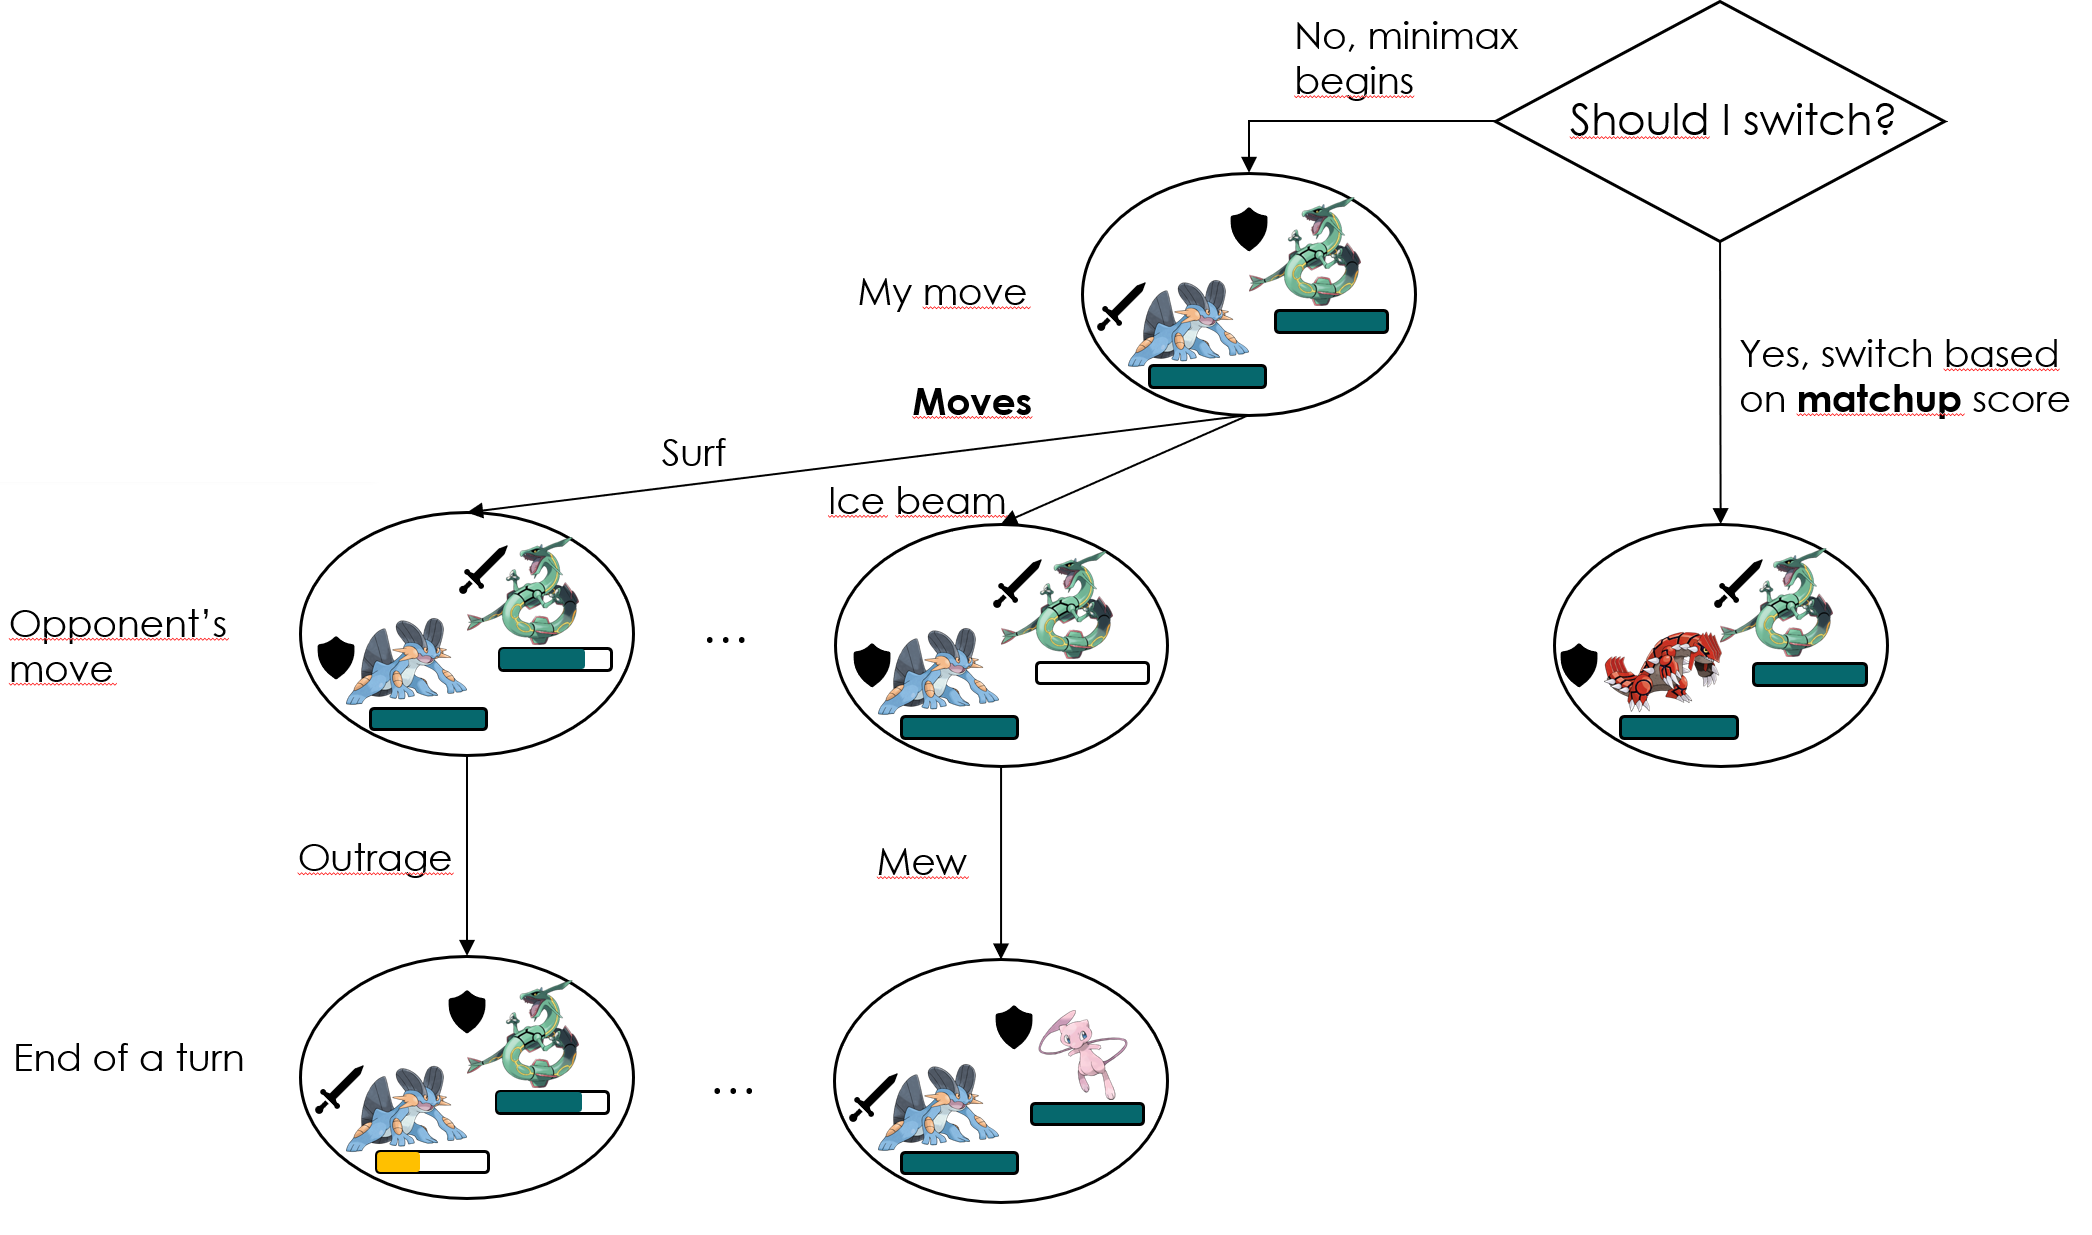
\includegraphics[width=0.8\textwidth]{images/minimax no switches.png}
    \caption{Minimax tree without switches.}
    \label{fig:minimax_without_switches}
\end{figure}

\end{document}
